\chapter{Implementation}
\label{cha:implementation}

\section{Tool Chain}
\label{sec:tc}
\begin{figure}[h!]
  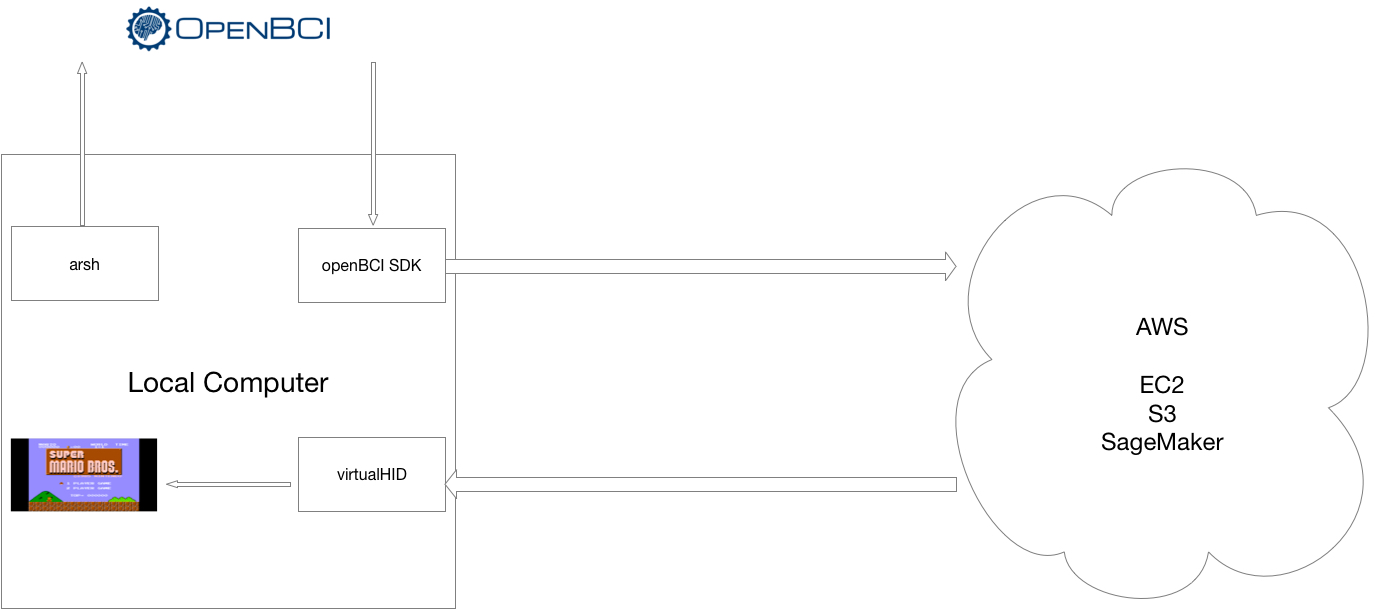
\includegraphics[width=\linewidth]{diagram.jpg}
  \caption{Tool Chain Diagram}
  \label{fig:tcd}
\end{figure}

Text about tool chain here
Figure \ref{fig:tcd}.

\section{Project work plan}
\label{sec:work-plan}

% Gantt chart in latex (requires pfggantt.sty file)
%%project Gantt chart


\begin{figure}
  \centering

  \begin{ganttchart}%
    [
    x unit = 0.25cm,
    y unit title=0.4cm,
    y unit chart=0.4cm,
    vgrid,
    title/.style={draw=black!50, fill=green!50!black},
    title label font=\sffamily\bfseries\color{white},
    title label anchor/.style={below=-1.6ex},
    title left shift=.05,
    title right shift=-.05,
    title height=1,
    bar/.style={draw=none, fill=blue!75},
    bar height=.6,
    bar label font=\small\color{black!50},
    milestone label font=\small\color{red!50},
    group right shift=0,
    group top shift=.6,
    group height=.3,
    group peaks={}{}{.2},
    incomplete/.style={fill=red}]{60}
    
    \gantttitle{ACRONYM}{60} \\
    \gantttitle{Year 1}{12} 
    \gantttitle{Year 2}{12} 
    \gantttitle{Year 3}{12}  
    \gantttitle{Year 4}{12}  
    \gantttitle{Year 5}{12} \\ 
    
    \ganttchartdata % data generated by the ICTProposal.cls
    
  \end{ganttchart}

  \caption[Gantt chart]{Project Gantt chart.}
  \label{fig:gantt}
\end{figure}


\subsection{Work package description}
\label{sec:wps}

%Include work-packages as separate files
%%%%%%%%%%%%%%%%%%%%%%%%%%%%%%
%  Work Package Description  %
%%%%%%%%%%%%%%%%%%%%%%%%%%%%%%

\begin{workpackage}{Virtual HID, Data Collection, and ML Code}
  \label{wp:data} %change and use appropriate description

  %%%%%%%%%%%%%%%%%% TOP TABLE %%%%%%%%%%%%%%%%%%%%%%%%%%%%%
  % Data for the top table
  \wpstart{1} %Starting Week
  \wpend{36} %End Week
  \wptype{Activity type} %RTD, DEM, MGT, or OTHER

  % Person Weeks per participant (required, max 7, * for leader)  
  % syntax: \personweeks{Participant number}{value}    (not wp leader)
  %     or  \personweeks{Participant short name}{value} (not wp leader)
  %         \personweeks*{Participant number}{value}    (wp leader)
  % for example:
  \personweeks*{georgio}{12}
  % etc.

  \makewptable % Work package summary table
    
  % Work Package Objectives
  \begin{wpobjectives}
    This work package has the following objectives:
    \begin{enumerate}
    \item To develop a Virtual Human Interface Device;
    \item To develop an  API that gathers raw data from the Cyton board and feeds it 
to a CSV file;
    \item To write code needed to efficiently store and manage datasets;
    \item To write code needed to start training Model 1 on Command A.
    \end{enumerate}
  \end{wpobjectives}
  
  % Work Package Description
  \begin{wpdescription}
    % Divide work package into multiple tasks.
    % Use \wptask command
    % syntax: \wptask{leader}{contributors}{start-m}{end-m}{title}{description}   
 
    \wptask{georgio}{georgio}{1}{12}{Task1}{
      \label{task:wp1task1}
      Here we will test the WP Task code. 
    }
    \wptask{georgio}{georgio}{6}{9}{Task2}{
      \label{task:wp2task2}
      In this task UZH will integrate the work done in ~\ref{task:wp1test}.
    }    
    \wptask{georgio}{All other}{9}{12}{Task3}{
      Here all the WP participants will apply the results to...

    }

    
  \end{wpdescription}
  
  % Work Package Deliverable
  \begin{wpdeliverables}
    % Data for the deliverables and milestones  tables
    % syntax: \deliverable[delivery date]{nature}{dissemination
    % level}{description} 
    %
    % nature: R = Report, P = Prototype, D = Demonstrator, O = Other
    % dissemination level: PU = Public, PP = Restricted to other
    % programme participants (including the Commission Services), RE =
    % Restricted to a group specified by the consortium (including the
    % Commission Services), CO = Confidential, only for members of the
    % consortium (including the Commission Services).
    % 
    % \wpdeliverable[date]{R}{PU}{A report on \ldots}

    \wpdeliverable[36]{georgio}{R}{PU}{Report on the definition of the model
      specifications.}\label{dev:wp1specs}
    
    \wpdeliverable[12]{georgio}{R}{PU}{Report on Feasibility study for the model
      implementation.}\label{dev:wp1implementation}

    \wpdeliverable[24]{georgio}{R}{PU}{Prototype of model
      implementation.}\label{dev:wp1prototype}

  \end{wpdeliverables}
\end{workpackage}
%%% Local Variables:
%%% mode: latex
%%% TeX-master: "proposal-main"
%%% End:
             %Use \input for first WP
%%%%%%%%%%%%%%%%%%%%%%%%%%%%%%
%  Work Package Description  %
%%%%%%%%%%%%%%%%%%%%%%%%%%%%%%

\begin{workpackage}{Model 1 Command A}
  \label{wp:m1cA} %change and use appropriate description

  %%%%%%%%%%%%%%%%%% TOP TABLE %%%%%%%%%%%%%%%%%%%%%%%%%%%%%
  % Data for the top table
  \wpstart{2} %Starting Week
  \wpend{36} %End Week
  \wptype{Activity type} %RTD, DEM, MGT, or OTHER

  % Person Weeks per participant (required, max 7, * for leader)  
  % syntax: \personweeks{Participant number}{value}    (not wp leader)
  %     or  \personweeks{Participant short name}{value} (not wp leader)
  %         \personweeks*{Participant number}{value}    (wp leader)
  % for example:
  \personweeks*{georgio}{3}  % etc.

  \makewptable % Work package summary table
    
  % Work Package Objectives
  \begin{wpobjectives}
    \begin{enumerate}
    \item To collect training, validation, and test datasets for 
Model 1 Command A; 
    \item Training Model 1 using aforementioned data;
    \item Testing/Patching Model 1.
    \end{enumerate}
  \end{wpobjectives}
  
  % Work Package Description
  \begin{wpdescription}
    % Divide work package into multiple tasks.
    % Use \wptask command
    % syntax: \wptask{leader}{contributors}{start-m}{end-m}{title}{description}   
 
    Description of work carried out in WP, broken down into tasks, and
    with role of partners list. Use the \texttt{\textbackslash wptask} command.

    \wptask{georgio}{georgio}{1}{12}{Task1}{
      \label{task:wp2task1}
      Here we will test the WP Task code. 
    }
    \wptask{georgio}{georgio}{6}{9}{Task2}{
      \label{task:wp2task2}
      In this task UZH will integrate the work done in ~\ref{task:wp2test}.
    }    
    \wptask{georgio}{All other}{9}{12}{Task 3}{
      Here all the WP participants will apply the results to...
    }
    
   
  \end{wpdescription}
  
  % Work Package Deliverable
  \begin{wpdeliverables}
    % Data for the deliverables and milestones  tables
    % syntax: \deliverable[delivery date]{nature}{dissemination
    % level}{description} 
    %
    % nature: R = Report, P = Prototype, D = Demonstrator, O = Other
    % dissemination level: PU = Public, PP = Restricted to other
    % programme participants (including the Commission Services), RE =
    % Restricted to a group specified by the consortium (including the
    % Commission Services), CO = Confidential, only for members of the
    % consortium (including the Commission Services).
    % 
    % \wpdeliverable[date]{R}{PU}{A report on \ldots}

    \wpdeliverable[36]{georgio}{R}{PU}{Report on the definition of the model
      specifications.}\label{dev:wp2specs}
    
    \wpdeliverable[12]{georgio}{R}{PU}{Report on Feasibility study for the model
      implementation.}\label{dev:wp2implementation}

    \wpdeliverable[24]{georgio}{R}{PU}{Prototype of model
      implementation.}\label{dev:wp2prototype}

  \end{wpdeliverables}

\end{workpackage}


%%% Local Variables:
%%% mode: latex
%%% TeX-master: "proposal-main"
%%% End:

%%%%%%%%%%%%%%%%%%%%%%%%%%%%%%
%  Work Package Description  %
%%%%%%%%%%%%%%%%%%%%%%%%%%%%%%

\begin{workpackage}{Model 1 n Commands}
  \label{wp:m1cN} %change and use appropriate 
description

  %%%%%%%%%%%%%%%%%% TOP TABLE %%%%%%%%%%%%%%%%%%%%%%%%%%%%%
  % Data for the top table
  \wpstart{1} %Starting Week
  \wpend{36} %End Week
  \wptype{Activity type} %RTD, DEM, MGT, or OTHER

  % Person Weeks per participant (required, max 7, * for leader)  
  % syntax: \personweeks{Participant number}{value}    (not wp leader)
  %     or  \personweeks{Participant short name}{value} (not wp leader)
  %         \personweeks*{Participant number}{value}    (wp leader)
  % for example:
  \personweeks*{UoP3}{12}
  % etc.

  \makewptable % Work package summary table
    
  % Work Package Objectives
  \begin{wpobjectives}
    This work package has the following objectives:
    \begin{enumerate*}
    \item Link the output from the Model to the virtual HID created in WP1;
    \item Map trigger thoughts to button presses; 
    \item Play a game of 1P Super Mario Bros.
    \end{enumerate*}
  \end{wpobjectives}
  
  % Work Package Description
  \begin{wpdescription}
    % Divide work package into multiple tasks.
    % Use \wptask command
    % syntax: \wptask{leader}{contributors}{start-m}{end-m}{title}{description}   
 
    Description of work carried out in WP, broken down into tasks, and
    with role of partners list. Use the \texttt{\textbackslash wptask} command.

    \wptask{UoC}{UoC}{1}{12}{Test}{
      \label{task:wp3test}
      Here we will test the WP Task code. 
    }
    \wptask{UoC}{UoC}{6}{9}{Integrate}{
      \label{task:wp3integrate}
      In this task UZH will integrate the work done in ~\ref{task:wp3test}.
    }    
    \wptask{UoP3}{All other}{9}{12}{Apply}{
      Here all the WP participants will apply the results to...
    }
    
    \paragraph{Role of partners}
    \begin{description*}
    \item[Participant short name] will lead Task~\ref{task:wp3integrate}.
    \item[UoC] will..
    \end{description*}
  \end{wpdescription}
  
  % Work Package Deliverable
  \begin{wpdeliverables}
    % Data for the deliverables and milestones  tables
    % syntax: \deliverable[delivery date]{nature}{dissemination
    % level}{description} 
    %
    % nature: R = Report, P = Prototype, D = Demonstrator, O = Other
    % dissemination level: PU = Public, PP = Restricted to other
    % programme participants (including the Commission Services), RE =
    % Restricted to a group specified by the consortium (including the
    % Commission Services), CO = Confidential, only for members of the
    % consortium (including the Commission Services).
    % 
    % \wpdeliverable[date]{R}{PU}{A report on \ldots}

    \wpdeliverable[36]{UoC}{R}{PU}{Report on the definition of the model
      specifications.}\label{dev:wp3specs}
    
    \wpdeliverable[12]{UoP3}{R}{PU}{Report on Feasibility study for the model
      implementation.}\label{dev:wp3implementation}

    \wpdeliverable[24]{UoP2}{R}{PU}{Prototype of model
      implementation.}\label{dev:wp3prototype}

  \end{wpdeliverables}

\end{workpackage}


%%% Local Variables:
%%% mode: latex
%%% TeX-master: "proposal-main"
%%% End:

%%%%%%%%%%%%%%%%%%%%%%%%%%%%%%
%  Work Package Description  %
%%%%%%%%%%%%%%%%%%%%%%%%%%%%%%

\begin{workpackage}{Model 2 n Commands}
  \label{wp:m2cN} %change and use appropriate 
description

  %%%%%%%%%%%%%%%%%% TOP TABLE %%%%%%%%%%%%%%%%%%%%%%%%%%%%%
  % Data for the top table
  \wpstart{1} %Starting Week
  \wpend{36} %End Week
  \wptype{Activity type} %RTD, DEM, MGT, or OTHER

  % Person Weeks per participant (required, max 7, * for leader)  
  % syntax: \personweeks{Participant number}{value}    (not wp leader)
  %     or  \personweeks{Participant short name}{value} (not wp leader)
  %         \personweeks*{Participant number}{value}    (wp leader)
  % for example:
  \personweeks*{UoC}{12}
  % etc.

  \makewptable % Work package summary table
    
  % Work Package Objectives
  \begin{wpobjectives}
    This work package has the following objectives:
    \begin{enumerate}
    \item Replicate all steps in WP2 and WP3 so that we get a Model 2 for a different individual trained on n the same n Commands as Model 1;
    \item Play a game of 2P Super Mario Bros.
    \end{enumerate}
  \end{wpobjectives}
  
  % Work Package Description
  \begin{wpdescription}
    % Divide work package into multiple tasks.
    % Use \wptask command
    % syntax: \wptask{leader}{contributors}{start-m}{end-m}{title}{description}   
 
    \wptask{UoC}{UoC}{1}{12}{Task1}{
      \label{task:wp1task1}
      Here we will test the WP Task code. 
    }
    \wptask{UoC}{UoC}{6}{9}{Task2}{
      \label{task:wp2task2}
      In this task UZH will integrate the work done in ~\ref{task:wp1test}.
    }    
    \wptask{UoP3}{All other}{9}{12}{Task3}{
      Here all the WP participants will apply the results to...

    }

    
  \end{wpdescription}
  
  % Work Package Deliverable
  \begin{wpdeliverables}
    % Data for the deliverables and milestones  tables
    % syntax: \deliverable[delivery date]{nature}{dissemination
    % level}{description} 
    %
    % nature: R = Report, P = Prototype, D = Demonstrator, O = Other
    % dissemination level: PU = Public, PP = Restricted to other
    % programme participants (including the Commission Services), RE =
    % Restricted to a group specified by the consortium (including the
    % Commission Services), CO = Confidential, only for members of the
    % consortium (including the Commission Services).
    % 
    % \wpdeliverable[date]{R}{PU}{A report on \ldots}

    \wpdeliverable[36]{UoC}{R}{PU}{Report on the definition of the model
      specifications.}\label{dev:wp1specs}
    
    \wpdeliverable[12]{UoP3}{R}{PU}{Report on Feasibility study for the model
      implementation.}\label{dev:wp1implementation}

    \wpdeliverable[24]{UoP2}{R}{PU}{Prototype of model
      implementation.}\label{dev:wp1prototype}

  \end{wpdeliverables}
\end{workpackage}
%%% Local Variables:
%%% mode: latex
%%% TeX-master: "proposal-main"
%%% End:

%%%%%%%%%%%%%%%%%%%%%%%%%%%%%%
%  Work Package Description  %
%%%%%%%%%%%%%%%%%%%%%%%%%%%%%%

\begin{workpackage}{Optimizations}
  \label{wp:opt} %change and use appropriate 
description

  %%%%%%%%%%%%%%%%%% TOP TABLE %%%%%%%%%%%%%%%%%%%%%%%%%%%%%
  % Data for the top table
  \wpstart{1} %Starting Week
  \wpend{36} %End Week
  \wptype{Activity type} %RTD, DEM, MGT, or OTHER

  % Person Weeks per participant (required, max 7, * for leader)  
  % syntax: \personweeks{Participant number}{value}    (not wp leader)
  %     or  \personweeks{Participant short name}{value} (not wp leader)
  %         \personweeks*{Participant number}{value}    (wp leader)
  % for example:
  \personweeks*{UoC}{12}
  % etc.

  \makewptable % Work package summary table
    
  % Work Package Objectives
  \begin{wpobjectives}
    This work package has the following objectives:
    \begin{enumerate}
 \item Optimizing the code in such a way that a trigger thought is recognized 
in realtime.
    \end{enumerate}
  \end{wpobjectives}
  
  % Work Package Description
  \begin{wpdescription}
    % Divide work package into multiple tasks.
    % Use \wptask command
    % syntax: \wptask{leader}{contributors}{start-m}{end-m}{title}{description}   
 
    \wptask{UoC}{UoC}{1}{12}{Task1}{
      \label{task:wp1task1}
      Here we will test the WP Task code. 
    }
    \wptask{UoC}{UoC}{6}{9}{Task2}{
      \label{task:wp2task2}
      In this task UZH will integrate the work done in ~\ref{task:wp1test}.
    }    
    \wptask{UoP3}{All other}{9}{12}{Task3}{
      Here all the WP participants will apply the results to...

    }

    
  \end{wpdescription}
  
  % Work Package Deliverable
  \begin{wpdeliverables}
    % Data for the deliverables and milestones  tables
    % syntax: \deliverable[delivery date]{nature}{dissemination
    % level}{description} 
    %
    % nature: R = Report, P = Prototype, D = Demonstrator, O = Other
    % dissemination level: PU = Public, PP = Restricted to other
    % programme participants (including the Commission Services), RE =
    % Restricted to a group specified by the consortium (including the
    % Commission Services), CO = Confidential, only for members of the
    % consortium (including the Commission Services).
    % 
    % \wpdeliverable[date]{R}{PU}{A report on \ldots}

    \wpdeliverable[36]{UoC}{R}{PU}{Report on the definition of the model
      specifications.}\label{dev:wp1specs}
    
    \wpdeliverable[12]{UoP3}{R}{PU}{Report on Feasibility study for the model
      implementation.}\label{dev:wp1implementation}

    \wpdeliverable[24]{UoP2}{R}{PU}{Prototype of model
      implementation.}\label{dev:wp1prototype}

  \end{wpdeliverables}
\end{workpackage}
%%% Local Variables:
%%% mode: latex
%%% TeX-master: "proposal-main"
%%% End:

%%%%%%%%%%%%%%%%%%%%%%%%%%%%%%
%  Work Package Description  %
%%%%%%%%%%%%%%%%%%%%%%%%%%%%%%

\begin{workpackage}{Real Life Application}
  \label{wp:app} %change and use appropriate description


  %%%%%%%%%%%%%%%%%% TOP TABLE %%%%%%%%%%%%%%%%%%%%%%%%%%%%%
  % Data for the top table
  \wpstart{20} %Starting Week
  \wpend{30} %End Week
  \wptype{Activity type} %RTD, DEM, MGT, or OTHER

  % Person Weeks per participant (required, max 7, * for leader)  
  % syntax: \personweeks{Participant number}{value}    (not wp leader)
  %     or  \personweeks{Participant short name}{value} (not wp leader)
  %         \personweeks*{Participant number}{value}    (wp leader)
  % for example:
  \personweeks*{georgio}{10}
  % etc.

  \makewptable % Work package summary table
    
  % Work Package Objectives
  \begin{wpobjectives}
    This work package has the following objectives:
    \begin{enumerate}
    \item Implement cogniLink to work on a controller of a wheelchair, this task derives from cogniLink as a forked project;
    \item Initiate research about Locked-in syndrome: Find suitiable use-cases and patients.
    \end{enumerate}
  \end{wpobjectives}

  % Work Package Description
  \begin{wpdescription}
    % Divide work package into multiple tasks.
    % Use \wptask command
    % syntax: \wptask{leader}{contributors}{start-m}{end-m}{title}{description}   
 
    \wptask{georgio}{georgio}{20}{22}{Task1}{
      \label{task:wp6task1}
      First Fork of cogniLink.
      A wheelchair controller/helper that can be fed command data as a replacement to the virtual HID will be designed and implemented.
    }
    \wptask{georgio}{georgio}{20}{30}{Task2}{
      \label{task:wp6task2}
      Initiation of formal research about Locked-in syndrome, patients, and practical use-case scenarios.
    }  
  \end{wpdescription}
  
  % Work Package Deliverable
  \begin{wpdeliverables}
    % Data for the deliverables and milestones  tables
    % syntax: \deliverable[delivery date]{nature}{dissemination
    % level}{description} 
    %
    % nature: R = Report, P = Prototype, D = Demonstrator, O = Other
    % dissemination level: PU = Public, PP = Restricted to other
    % programme participants (including the Commission Services), RE =
    % Restricted to a group specified by the consortium (including the
    % Commission Services), CO = Confidential, only for members of the
    % consortium (including the Commission Services).
    % 
    % \wpdeliverable[date]{R}{PU}{A report on \ldots}

    \wpdeliverable[22]{georgio}{R}{PU}{Report about integration with wheelchair.}\label{dev:wp6f1report}
    
    \wpdeliverable[30]{georgio}{P}{PU}{Forking cogniLink and merging changes needed for wheelchair integration.}\label{dev:wp6fork}

    \wpdeliverable[30]{georgio}{R}{PU}{Report about research findings and future steps towards integrating with a locked in patient. }\label{dev:wp6r2research}

    \wpdeliverable[30]{georgio}{R}{PU}{Main Main Report update with full progress accomplished after the end of WP6.}\label{dev:MR0.6}
  
  \end{wpdeliverables}
\end{workpackage}
%%% Local Variables:
%%% mode: latex
%%% TeX-master: "proposal-main"
%%% End:

%%%%%%%%%%%%%%%%%%%%%%%%%%%%%%
%  Work Package Description  %
%%%%%%%%%%%%%%%%%%%%%%%%%%%%%%

\begin{workpackage}{Universal Model, n Commands}
  \label{wp:mUcN} %change and use appropriate 
description

  %%%%%%%%%%%%%%%%%% TOP TABLE %%%%%%%%%%%%%%%%%%%%%%%%%%%%%
  % Data for the top table
  \wpstart{1} %Starting Week
  \wpend{36} %End Week
  \wptype{Activity type} %RTD, DEM, MGT, or OTHER

  % Person Weeks per participant (required, max 7, * for leader)  
  % syntax: \personweeks{Participant number}{value}    (not wp leader)
  %     or  \personweeks{Participant short name}{value} (not wp leader)
  %         \personweeks*{Participant number}{value}    (wp leader)
  % for example:
  \personweeks*{UoC}{12}
  % etc.

  \makewptable % Work package summary table
    
  % Work Package Objectives
  \begin{wpobjectives}
    This work package has the following objectives:
    \begin{enumerate}
    \item To develop a Virtual Human Interface Device;
    \item To develop an  API that gathers raw data from the Cyton board and feeds it 
to a CSV file;
    \item To write code needed to efficiently store and manage datasets;
    \item To write code needed to start training Model 1 on Command A.
    \end{enumerate}
  \end{wpobjectives}
  
  % Work Package Description
  \begin{wpdescription}
    % Divide work package into multiple tasks.
    % Use \wptask command
    % syntax: \wptask{leader}{contributors}{start-m}{end-m}{title}{description}   
 
    \wptask{UoC}{UoC}{1}{12}{Task1}{
      \label{task:wp1task1}
      Here we will test the WP Task code. 
    }
    \wptask{UoC}{UoC}{6}{9}{Task2}{
      \label{task:wp2task2}
      In this task UZH will integrate the work done in ~\ref{task:wp1test}.
    }    
    \wptask{UoP3}{All other}{9}{12}{Task3}{
      Here all the WP participants will apply the results to...

    }

    
  \end{wpdescription}
  
  % Work Package Deliverable
  \begin{wpdeliverables}
    % Data for the deliverables and milestones  tables
    % syntax: \deliverable[delivery date]{nature}{dissemination
    % level}{description} 
    %
    % nature: R = Report, P = Prototype, D = Demonstrator, O = Other
    % dissemination level: PU = Public, PP = Restricted to other
    % programme participants (including the Commission Services), RE =
    % Restricted to a group specified by the consortium (including the
    % Commission Services), CO = Confidential, only for members of the
    % consortium (including the Commission Services).
    % 
    % \wpdeliverable[date]{R}{PU}{A report on \ldots}

    \wpdeliverable[36]{UoC}{R}{PU}{Report on the definition of the model
      specifications.}\label{dev:wp1specs}
    
    \wpdeliverable[12]{UoP3}{R}{PU}{Report on Feasibility study for the model
      implementation.}\label{dev:wp1implementation}

    \wpdeliverable[24]{UoP2}{R}{PU}{Prototype of model
      implementation.}\label{dev:wp1prototype}

  \end{wpdeliverables}
\end{workpackage}
%%% Local Variables:
%%% mode: latex
%%% TeX-master: "proposal-main"
%%% End:


\subsection{List of work packages}
\label{sec:wplist}
\makewplist

\subsection{List of deliverables}
\label{sec:deliverables}
\instructions{
\textbf{KEY}\\
\emph{Deliverable numbers in order of delivery dates. Please use the numbering convention $<$WP number$>.<$number of deliverable within that WP$>$.}
\vskip0.2cm
\noindent\emph{For example, deliverable 4.2 would be the second deliverable from work package 4.}
\vskip0.2cm
\noindent\textbf{Type:}\\
\emph{Use one of the following codes:}\\
\indent R: Document, report (excluding the periodic and final reports)\\
\indent DEM: Demonstrator, pilot, prototype, plan designs\\
\indent DEC: Websites, patents filing, press \& media actions, videos, etc.\\
\indent OTHER: Software, technical diagram, etc.
\vskip0.2cm
\noindent\textbf{Dissemination level}:\\
\emph{Use one of the following codes:}\\
\indent PU = Public, fully open, e.g. web\\
\indent CO = Confidential, restricted under conditions set out in Model Grant Agreement\\
\indent CI = Classified, information as referred to in Commission Decision 2001/844/EC.\\
\vskip0.2cm
\noindent\textbf{Delivery date}:\\
Measured in weeks from the project start date (week 1).
}
\makedeliverablelist

\clearpage
\section{Management and risk assessment}
\label{sec:management}
\setcounter{table}{0}
\instructions{
\begin{itemize}
\item Describe the organisational structure and the decision-making ( including a list of
milestones (table 3.2a))
\item Describe any critical risks, relating to project implementation, that the stated project's objectives may not be achieved. Detail any risk mitigation measures. Please provide a table with critical risks identified and mitigating actions (table 3.2b)
\end{itemize}
}



\subsection{List of milestones}
\label{sec:milestones}
\instructions{
\vskip0.2cm
\noindent\textbf{KEY}\\
\textbf{Estimated date}\\
\emph{Measured in weeks from the project start date (week 1)}
\vskip0.2cm
\noindent\textbf{Means of verification}\\
\emph{Show how you will confirm that the milestone has been attained. Refer to indicators if appropriate. For example: a laboratory prototype that is ‘up and running’; software released and validated by a user group; field survey complete and data quality validated.}}

\milestone[Week 6]{Completed Development of Model 1 for Command A}{Execution of command using trigger thought}{WP\,\ref{wp:m1cA}}
\milestone[Week 8]{Completed Development of Model 1 for Commands A and B}{Execution of alternating commands using trigger thoughts}{WP\,\ref{wp:m1cN}}
\milestone[Week 12]{Completed Development of Model 1 for n-Commnands}{Playing a game of 1P Super Mario Bros}{WP\,\ref{wp:m1cN}}
\milestone[Week 18]{Completed Development of Model 2 for n-Commnands}{Playing a game of 2P Super Mario Bros}{WP\,\ref{wp:m2cN}}
\milestone[Week 22]{Transitioning from using virtualHID on OpenEmu to Wheelchair in Realtime}{Driving a wheelchair with no hands}{WP\,\ref{wp:app}}
\milestone[Week 40]{Integration with Locked-in Patient}{Enabling a Locked-in patient to communicate using cogniLink}{WP\,\ref{wp:mUcN}}
\milestone[Week 40]{Training Universal Model for n-Commands}{Ease of training models for new users}{WP\,\ref{wp:mUcN}}
\makemilestoneslist

\subsection{Critical risks for implementation}
\label{sec:risks}

\criticalrisk{Not being able to recognize thoughts via brain activity in a timely manner.}{WP\,\ref{wp:data}}{Resort to using motor neurons.}
\criticalrisk{Difficulty in implementing the virtual HID using macOS' IOKit.}{WP\,\ref{wp:data}}{Resort to a different OS where the virutal HID would be implemented.}
\makerisklist

\clearpage

\section{List of Materials}
\begin{table}[]
  \caption{List of Materials}
  \label{my-label}
  \begin{tabular}{|l|l|
  >{\columncolor[HTML]{FFFFFF}}l |}
  \hline
  \cellcolor[HTML]{C0C0C0}{\color[HTML]{000000} \textbf{Name}}                                                                                                    & \cellcolor[HTML]{C0C0C0}{\color[HTML]{000000} \textbf{Cost (USD)}} & \cellcolor[HTML]{C0C0C0}{\color[HTML]{000000} \textbf{Link}} \\ \hline
  {\color[HTML]{000000} Ultracortex "Mark IV" EEG Headset}                                                                                                        & 999.99                                                             & {\color[HTML]{333333} {\ul hhttps://goo.gl/JRLunf}}           \\ \hline
  {\color[HTML]{000000} WiFi Shield}                                                                                                                              & 149.99                                                             & {\color[HTML]{333333} {\ul hhttps://goo.gl/9UTFpB}}           \\ \hline
  {\color[HTML]{000000} Cyton + Daisy Biosensing Boards (16-Channels)}                                                                                            & 949.99                                                             & {\color[HTML]{333333} {\ul hhttps://goo.gl/nDMBGQ}}           \\ \hline
  {\color[HTML]{000000} \begin{tabular}[c]{@{}l@{}}Energizer Rechargeable AA Batteries, NiMH,\\ 2000 mAh, Pre-Charged, 8 count (Recharge Universal)\end{tabular}} & 19.98                                                              & {\color[HTML]{333333} {\ul hhttps://goo.gl/qckQAb}}           \\ \hline
  {\color[HTML]{000000} Gold Cup Electrodes}                                                                                                                      & 29.99                                                              & {\color[HTML]{333333} {\ul hhttps://goo.gl/2eckXr}}           \\ \hline
  {\color[HTML]{000000} ELEFIX EEG Paste - 6 oz tube}                                                                                                             & 17.99                                                              & {\color[HTML]{333333} {\ul hhttps://goo.gl/LrkUg6}}           \\ \hline
  \cellcolor[HTML]{C0C0C0}\textbf{Total:}                                                                                                                         & \cellcolor[HTML]{C0C0C0}\textbf{2167.93}                           & \cellcolor[HTML]{C0C0C0}                                     \\ \hline
  \end{tabular}
  \end{table}
  